\documentclass[a4paper,12pt,oneside,final]{extarticle}
\usepackage[top=2cm, bottom=2cm, left=3cm, right=1cm]{geometry}
\usepackage{scrextend}

\usepackage[T2A,T1]{fontenc}
\usepackage[ukrainian,russian,english]{babel}
\usepackage{tempora}
\usepackage{fontspec}
\setmainfont{tempora}

\frenchspacing

% Lists
\usepackage{enumitem}
\renewcommand\labelitemi{--}
\renewcommand\labelenumi{\arabic*}
\setlist[description]{noitemsep,style=multiline,leftmargin=2.5cm}
\setlist[itemize]{noitemsep, topsep=0pt}
\setlist[enumerate]{noitemsep, topsep=0pt}

\usepackage{titlesec}
\newcommand{\sectionbreak}{\clearpage}

\usepackage{hyperref} % make refs clickable
\usepackage{float}
\usepackage{pgfplots}
\usepackage{graphicx}
\usepackage{multirow}
\usepackage{amssymb,amsfonts,amsmath,amsthm}
\usepackage{csquotes}
\usepackage{xstring}

\numberwithin{equation}{section}

\usepackage{listings}
\lstset{basicstyle=\footnotesize\ttfamily,breaklines=true}
\lstset{language=Matlab}

\makeatletter
\def\maxwidth#1{\ifdim\Gin@nat@width>#1 #1\else\Gin@nat@width\fi}
\makeatother

\begin{document}
\Russian
\title{Основы управление развитием организации}
\maketitle
\tableofcontents

%
% section 1
%
\section{Модуль I}
\subsection{Понятие и сущность управления}

\subsection{Управление и менеджеры}

\subsection{Развитие теории и практики управления. Современная система взглядов на управление}

\subsection{Определение <<организационная система>>. Организационные системы как системы междисциплинарной природы}

\subsection{Внутренняя и внешняя среда организационной системы}
Внутренняя среда организационной системы --- это ее организационное строение и ситуационные факторы внутри нее (внутренние переменные).
К основным переменным относятся: структура, цели, задачи, технологии и люди.

Производство --- это средства и предметы труда, а также трудовые ресурсы.

Внешняя среда организации --- это силы внешние по отношению к организации, которые действуют на ее результативность. 
Факторы, оказывающие немедленное воздействие или влияние на организацию --- это среда прямого воздействия, а все другие --- косвенного.

Выделяют 4 (четыре) основных свойства внешней среды: 
\begin{itemize}
	\item взаимосвязанность факторов внешней среды (уровень силы, с которой изменение одного фактора воздействует на другие); 
	\item сложность внешней среды (количество факторов и уровень вариативности); 
	\item подвижность среды (скорость, с которой могут меняться факторы); 
	\item неопределенность среды (является функцией количества информации, которой располагает организация по поводу конкретного факторы, а также функция уверенности в этой информации). 
\end{itemize}

\subsection{Задачи управления организационными системами}

\subsection{Понятие принципа и роль в управлении организационной системой}

\subsection{Содержание основных принципов управления}

\subsection{Цели организационных систем и их классификация}

\subsection{Понятие об управленческом цикле}

\subsection{Характеристика функций управления}

\subsection{Понятие коммуникаций и их роль в системе управления}

\subsection{Процесс коммуникаций: модель, основные этапы и элементы}

\subsection{Понятие и основные элементы процесса управления}

\subsection{Управленческое решение. Этапы и процедуры процесса принятия решений}

\subsection{Необходимость моделирования. Обзор моделей науки управления}

\subsection{Общенаучные методы}

\subsection{Конкретные или специфические методы управления}

\subsection{Сущность и смысл контроля}

\subsection{Процесс контроля}

\subsection{Характеристики эффективного контроля}

%
% section 2
%
\section{Модуль II}
\subsection{Концепция управления персоналом}

\subsection{Принципы управления персоналом}

\subsection{Методы построения системы управления персоналом}

\subsection{Методы управления персоналом}

\subsection{Источники организации найма персонала}

\subsection{Требования к кандидатам на замещение вакантной должности}

\subsection{Организация процесса отбора претендентов на вакантную должность}

\subsection{Сущность и виды профориентации и адаптации персонала}

\subsection{Опыт профориентации и адаптации персонала}

\subsection{Организация управления профориентацией и адаптацией персонала}

\subsection{Изучение состояния работы по профориентации и адаптации персонала}

\subsection{Группы и их значимость}

\subsection{Управление неформальной организацией }

\subsection{Повышение эффективности работы групп. Факторы, влияющие на эффективность деятельности групп и организации}

\subsection{Власть, влияние}

\subsection{Убеждение и участие}

\subsection{Основы лидерства}

\subsection{Традиционные концепции лидерства}

\subsection{Концепции ситуационного лидерства}

\subsection{Новое в теориях лидерства}

\subsection{Природа конфликта и стресса}
Конфликт --- это отсутствие согласия между двумя и более сторонами, которыми могут быть как конкретные лица, группы, так и организации в целом, причем это несогласие между сторонами приводит к тому, что сознательное поведение одной из сторон вступает в противоречие с интересами другой стороны.

Причины: распределение ресурсов, взаимозависимость задач, различие в целях, различие в представлениях и ценностях, различие в манерах поведения и жизненном опыте и неудовлетворительных коммуникациях.

Типы конфликтов:
\begin{itemize}
	\item внутриличностный;
	\item межличностный;
	\item между личностью и группой;
	\item внешний.
\end{itemize}

Позитивные функции конфликта.
\begin{itemize}
	\item разрядка напряженности между сторонами;
	\item сплочение коллектива перед внешним врагом. Широко известно, что дружить легче против кого-то;
	\item несомненно, внешний враг может помочь усилению консолидации членов группы;
	\item получение новой информации об оппоненте и окружающей социальной среде;
	\item большая расположенность к сотрудничеству в будущем;
	\item снятие синдрома покорности у подчиненных.
\end{itemize}

Негативные функции конфликта.
\begin{itemize}
	\item большие эмоциональные и материальные затраты на участие в конфликте;
	\item рост неудовлетворенности, плохое моральное состояние;
	\item снижение производительности труда, рост текучести кадров;
	\item представление о второй стороне как о враге;
	\item уменьшение сотрудничества после завершения конфликта;
	\item сложное восстановление деловых отношений (<<шлейф>> конфликта);
	\item усиление тенденции к авторитарному руководству.
\end{itemize}

\subsection{Управление конфликтной ситуацией}
% http://www.nnre.ru/delovaja_literatura/menedzhment_konspekt_lekcii/p12.php
Управление конфликтом --- это целенаправленное воздействие на устранение причин конфликта или на коррекцию поведения участников. 
Методы управления и разрешения конфликтов делятся на три группы: внутриличностные, структурные и межличностные.

Внутриличностные методы воздействуют на отдельную личность и состоят в правильной организации своего собственного поведения, в умении высказывать свою точку зрения, не вызывая защитной реакции со стороны оппонента.

Структурные методы изменяют структуру заданий работникам или структуру организации. К структурным методам разрешения конфликтов относятся следующие:
\begin{enumerate}
	\item Разъяснение требований к работе. 
	\item Использование координационных и интеграционных механизмов, которые улучшают согласованность между подразделениями и отдельными людьми.
	\item Постановка общеорганизационных целей.
	\item Использование системы вознаграждений для поощрения поведения, направленного на избежание негативных последствий конфликтов.
\end{enumerate}

Методы разрешения межличностных конфликтов через сотрудничество:
\begin{enumerate}
	\item Определите проблему в категориях целей, а не решений.
	\item После того, как проблема определена, определите решения, которые приемлемы для обеих сторон.
	\item Сосредоточьте внимание на проблеме, а не на личных качествах другой стороны.
	\item Создайте атмосферу доверия, увеличив взаимное влияние и обмен информацией.
	\item Во время общения создайте положительное отношение друг к другу, проявляя симпатию и выслушивая мнения другой стороны, а также сводя к минимуму проявления гнева и угроз.
\end{enumerate}

\subsection{Управление изменениями}
Управление изменениями --- это структурный подход к переводу индивидов, команд и организаций из текущего состояния в желаемое будущее состояние. 
Целью этого организационного процесса является расширение прав и возможностей сотрудников принять и поддержать изменения в их текущем бизнес-окружении. 
В управлении проектами, управление изменениями рассматривается как процесс управления проектом, в котором формально представлены и одобрены изменения проекта.

В управлении изменениями используются различные подходы для анализа, подготовки и проведения изменений:
\begin{enumerate}
	\item Индивидуальные изменения.
	\item Командные изменения.
	\item Организационные изменения.
\end{enumerate}

Использование типовых шагов для проведения изменений подробно рассмотрено в работах Коттера, таких как:
\begin{enumerate}
	\item Преодоление состояния удовлетворенности текущей ситуацией.
	\item Формирование команды для проведения изменения.
	\item Определение видения желаемого будущего и стратегии перехода.
	\item Широкое информирование о проводимых изменениях.
	\item Устранение препятствий и барьеров, мешающих проведению изменений.
	\item Достижение быстрых первых успехов.
	\item Поддержание процесса изменений с целью недопущения отката назад.
	\item Закрепление проведенных изменений в корпоративной культуре.
\end{enumerate}

Управление изменениями оперирует такими понятиями, как лидерство, эффективность коммуникаций и принятие потребности в изменениях для разработки точных стратегий перехода, для того чтобы преодолеть неизбежное сопротивление переменам.

\subsection{Сущность, функции и элементы маркетинга}
Маркетинг --- это комплексная система организации производства и сбыта, ориентированная на возможное более полное удовлетворение быстро меняющихся и все более разнообразных потребностей потребителей посредством рынка и получение на этой основе устойчивой прибыли и конкурентных преимуществ.

Выделяют 3 (три) подхода к определению сущности маркетинга:
\begin{itemize}
	\item как самостоятельный вид производственной деятельности;
	\item как функция управления;
	\item как современное видение философии бизнеса.
\end{itemize}

Концепция маркетинга --- это философия управления, которая способствует получению товара производителями прибыли посредством удовлетворения потребностей потребителей.

% http://www.grandars.ru/student/marketing/funkcii-marketinga.html
Главные функции маркетинга:
\begin{itemize}
	\item аналитическая функция;
	\item продуктово-производственная функция;
	\item сбытовая функция (функция продаж);
	\item функция управления и контроля.
\end{itemize}

Комплекс маркетинга --- совокупность управляемых элементов маркетинговой деятельности организации, манипулируя которыми она старается наилучшим образом удовлетворить потребности целевых рынков.
% https://ru.wikipedia.org/wiki/%D0%A2%D0%B5%D0%BE%D1%80%D0%B8%D1%8F_4P
Теория 4P \textit{(маркетинг-микс)} — маркетинговая теория, основанная на четырёх основных <<координатах>> маркетингового планирования:
\begin{description}
	\item[Product] Товар или услуга, ассортимент, качество, свойства товара, дизайн и эргономика.
	\item[Price] Цена, наценки, скидки.
	\item[Promotion] Продвижение, реклама, пиар, стимулирование сбыта.
	\item[Place] Месторасположения торговой точки, каналы распределения, персонал продавца.
\end{description}

\subsection{Задачи, виды и структура маркетинговых исследований}
Маркетинговое исследование --- это систематический поиск, сбор, анализ и представление данных и сведений, относящихся к конкретной рыночной ситуации, с которой пришлось столкнуться предприятию. 
Маркетинговое исследование можно также определить как систематический сбор, учет и анализ данных по маркетингу и маркетинговым проблемам в целях совершенствования качества процедур принятия решений и контроля в маркетинговой среде. 
Имеется целый ряд аналогичных и иных определений маркетинговых исследований.

Основные цели маркетингового исследования:
\begin{itemize}
	\item уменьшить неопределенность и минимизировать риск в процессе принятия управленческих решений;
	\item следить за процессом реализации маркетинговых задач.
\end{itemize}

Глобальные цели маркетингового исследования --- это информационное обеспечение маркетинга, то есть сбор необходимой информации и аналитическое обеспечение, заключающееся в использовании математических моделей для анализа данных и получения с их помощью прогнозов и возможности принятия оптимальных решений.

% http://works.doklad.ru/view/hARiKdLaWJM.html
Задачи маркетинговых исследований могут быть самыми разнообразными и диктоваться потребностями разработки стратегии маркетинга, формирование ценовой, товарной, коммуникационной, сбытовой политики и другими аспектами управления маркетингом на предприятии. 
Наиболее типичные решаемые задачи маркетинговых исследований:
\begin{itemize}
	\item изучение характеристик рынка;
	\item замеры потенциальных возможностей рынка;
	\item анализ распределения долей рынка между фирмами;
	\item анализ сбыта;
	\item изучение тенденций деловой активности;
	\item изучение товаров конкурентов;
	\item краткосрочное прогнозирование;
	\item изучение реакции на новый товар и его потенциала;
	\item долгосрочное прогнозирование;
	\item изучение политики цен.
\end{itemize}

\begin{figure}[h]
	\centering
	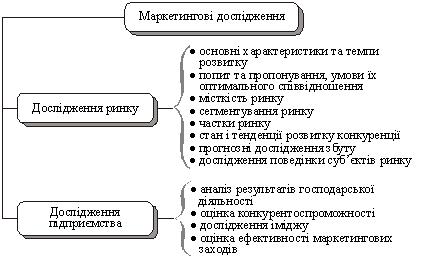
\includegraphics[width=\maxwidth{\textwidth}]{management-figures/marketing_structure}
	\caption{Структура маркетинговых исследований}
\end{figure}

Типы маркетинговых исследований:
\begin{enumerate}
	\item Разведочные или поисковые, предшествующие разработке программы основного исследования. 
	Предпринимаются для сбора предварительной информации, освещающие проблемы, позволяет выдвинуть гипотезы.
	\item Описательные \textit{(дескриптивные)}. 
	Имеющие целью констатацию реальных фактов, событий, показателей, полученных в результате сбора информации. 
	\item Экспериментальные. 
	Проводится с целью проверки выдвинутой гипотезы.
	\item Аналитические. 
	Проводимое для выявления и моделирования связи и деятельности фирмы с факторами окружающей среды. 
\end{enumerate}

\subsection{Маркетинговое сегментирование рынка}
Сегментирование рынка --- это процесс разделения рынка на отдельные части --- сегменты, отличающиеся друг от друга разными возможностями сбыта.

Сегмент рынка --- это особым образом выделенная часть рынка, группы потребителей или предприятий, обладающих определенными общими признаками. 
Может быть осуществлено по множеству критериев --- мерилам оценки обоснованности выбора сегмента рынка. 
Принцип сегментирования --- показатель выделения данного сегмента рынка. 

\begin{figure}[h]
	% http://powerbranding.ru/segmentirovanie/osnovy/
	\centering
	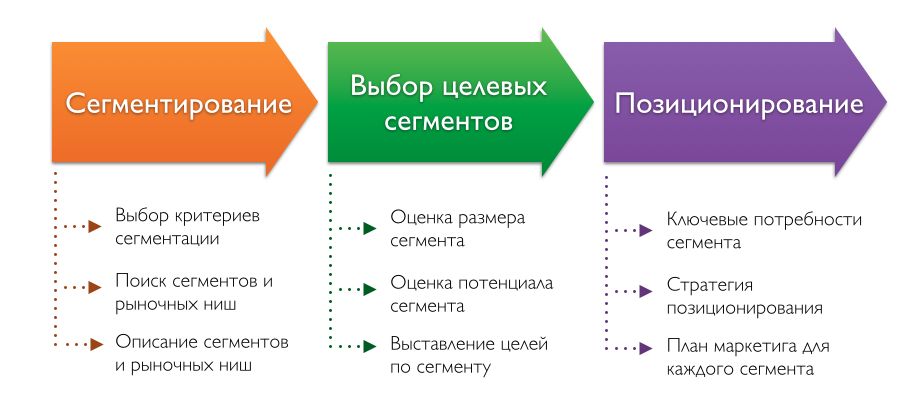
\includegraphics[width=\maxwidth{\textwidth}]{management-figures/marketing_segmentation_process}
	\caption{Схема сегментации рынка}
\end{figure}

Могут быть использованы следующие критерии:
\begin{enumerate}
	\item Различия между потребителями позволяющее объединить их в один сегмент.
	\item Сходство, формирующие устойчивость.
	\item Наличие показателей, позволяющих измерить характеристики и требования потребителей, определить емкость рынка.
	\item Возможность выстоять в конкурентной борьбе.
	\item Достаточность объема продаж.
	\item Доступность сегмента для предприятия.
\end{enumerate}

Существует три варианта охвата рынка:
\begin{itemize}
	\item недифференцированный маркетинг;
	\item дифференцированный маркетинг;
	\item концентрированный маркетинг.
\end{itemize}

На выбор стратегии охвата рынка влияют ресурсы фирмы, степень однородности продукции, этапы жизненного цикла товара, степень однородности рынка.

Обобщенные критерии правильного определения сегмента:
\begin{itemize}
\item доступность;
\item измеримость;
\item значимость по размерам, динамике спроса и своему совокупному потенциалу;
\item заметные отличия от других составных частей рынка;
\item относительная устойчивость сходства спроса со стороны потребителей.
\end{itemize}

\subsection{Цель и суть товарной политики}
Товарная политика --- это совокупность решений, касающихся формирования эффективной рыночно-ориентированной производственной программы предприятия.

Товарная политика ­­--- область целенаправленных действий по отдельным предложенным для использования товарам и услугам (вид, количество, свойство и т.д.), а также по совокупности отдельных продуктов (ширина, глубина, структура ассортимента).

Цель товарной политики --- добиться сбалансированного товарного ассортимента и конкурентоспособности каждого отдельного продукта, а так же:
\begin{itemize}
	\item обеспечение прибыли;
	\item увеличение товарооборота;
	\item увеличение доли рынка;
	\item снижение расходов на производство и маркетинг;
	\item повышение имиджа;
	\item рассеивание риска.
\end{itemize}

Задачи товарной политики --- принятие решений в области предлагаемых предприятием товаров, касающихся самих продуктов, их присутствия на рынке, а также связанных с этим решений по производственной программе.

\subsection{Использование средств стимулирования сбыта}
% http://www.aup.ru/books/m99/7_9.htm
Стимулирование сбыта – это совокупность приемов, применяемых на протяжении всего жизненного цикла товара в отношении трех участников рынка (потребителя, оптового торговца, продавца), для краткосрочного увеличения объема сбыта, а также для увеличения числа новых покупателей.

Стимулирование сбыта имеет многоцелевую направленность: потребитель, продавец, торговый посредник.

Выбор средств стимулирования зависит от поставленных целей. 
Все средства можно объединить в три большие группы:
\begin{itemize}
	\item предложение цены (продажа по сниженным ценам, льготные купоны, талоны, дающие право на скидку);
	\item предложение в натуральной форме (премии, образцы товара);
	\item активное предложение (конкурсы покупателей, игры, лотереи).
\end{itemize}

Процесс выбора комплекса продвижения товара включает этапы:
\begin{enumerate}
	\item Определение цели продвижения. 	
	\begin{enumerate}
		\item Информирование потребителей.
		\item Стимулирование сбыта.
		\item Формирование благоприятного имиджа.
		\item Влияние на привычки потребителей.
		\item Поддержание деловых отношений, взаимопонимание с деловыми партнерами и т.д.
	\end{enumerate}
	\item Оценивание факторов, влияющих на комплекс продвижения.		
	\begin{enumerate}
		\item Цели фирмы.
		\item Стратегия.
		\item Целевая аудитория.
		\item Тип товара.
		\item Этап жизненного цикла.
		\item Объем рынка.
		\item Стоимость.
	\end{enumerate}
	\item Разработка стратегии продвижения.	
	\begin{enumerate}
		\item Интенсификация рекламы.
		\item Новая рекламная компания.
	\end{enumerate}
	\item Составление и распределение бюджета распределения.	
	\begin{enumerate}
		\item <<Снизу-вверх>>. Общая сумма затрат на комплекс продвижения.
		\item <<Сверху-вниз>>. Составляем статьи отдельно для рекламы, персональной продажи, а потом считаем общую сумму.
	\end{enumerate}
	\item Методы составления бюджета.	
	\item Оценивание комплекса продвижения.	
\end{enumerate}

\subsection{Ценовая политика в маркетинговой деятельности. Методы расчета и установления цены}
Цена --- денежное выражение стоимости товара, предназначенное для непрямого измерения общественно-необходимых затрат рабочего времени на производство товара. Количество денежных единиц, которые должен заплатить покупатель продавцу за весь товар или его единицу.

Ценовая политика --- это установление определенных цен и способов маневрирование ими в зависимости от положения на рынке, которые позволяют овладеть долю рынка, получить расчетную прибыль, а также решить другие стратегические и оперативные задачи.

На цену влияют внешние факторы (политическая стабильность страны, экономика, гос. регулирование цены, состояние рынка) и внутренний (стратегия и тактика фирмы, специфика жизненного цикла товара, особенности производства и характеристики системы продвижения товаров на рынке).

Алгоритм определение цены:
\begin{enumerate}
	\item Определение целей. 	
	\item Определение и анализ спроса. 	
	\item Анализ издержек производства. 	
	\item Анализ цен товаров конкурентов. 	
	\item Методы ценообразования. 	
	\item Выбор ценовой стратегии. 	
	\item Адаптация цен. 	
\end{enumerate}

Методы ценообразования:
\begin{itemize}
	\item ориентированный на затратах;
	\item ориентированная на спрос;
	\item ориентируемые на конкурентов.
\end{itemize}

\end{document}